\subsection{Implementación de la API para la Generación de Imágenes}

Uno de los objetivos principales del proyecto fue desarrollar un sistema que permitiera la generación de imágenes a partir de descripciones textuales, accesible desde la plataforma JMR. Para ello, se implementó una API REST utilizando el framework \textit{FastAPI}, desplegada en local mediante Docker. Esta solución actúa como puente entre el sistema generativo y la interfaz de usuario, facilitando la separación de responsabilidades y permitiendo futuras ampliaciones sin comprometer la estabilidad del entorno principal.

\subsubsection{Arquitectura de la API}

La API está diseñada para ser modular, escalable y fácilmente integrable en otros sistemas. Su estructura se organiza en varios módulos independientes:

\begin{itemize}
\item \textbf{Módulo de generación de imágenes}: Encargado de cargar el modelo seleccionado y generar imágenes a partir de un prompt textual.
\item \textbf{Módulo de gestión de modelos}: Permite la subida, eliminación y listado de modelos de generación disponibles en el sistema.
\item \textbf{Interfaz RESTful}: Define los distintos endpoints disponibles para interactuar con la API, conforme al paradigma CRUD.
\end{itemize}

\begin{figure}[H]
\centering
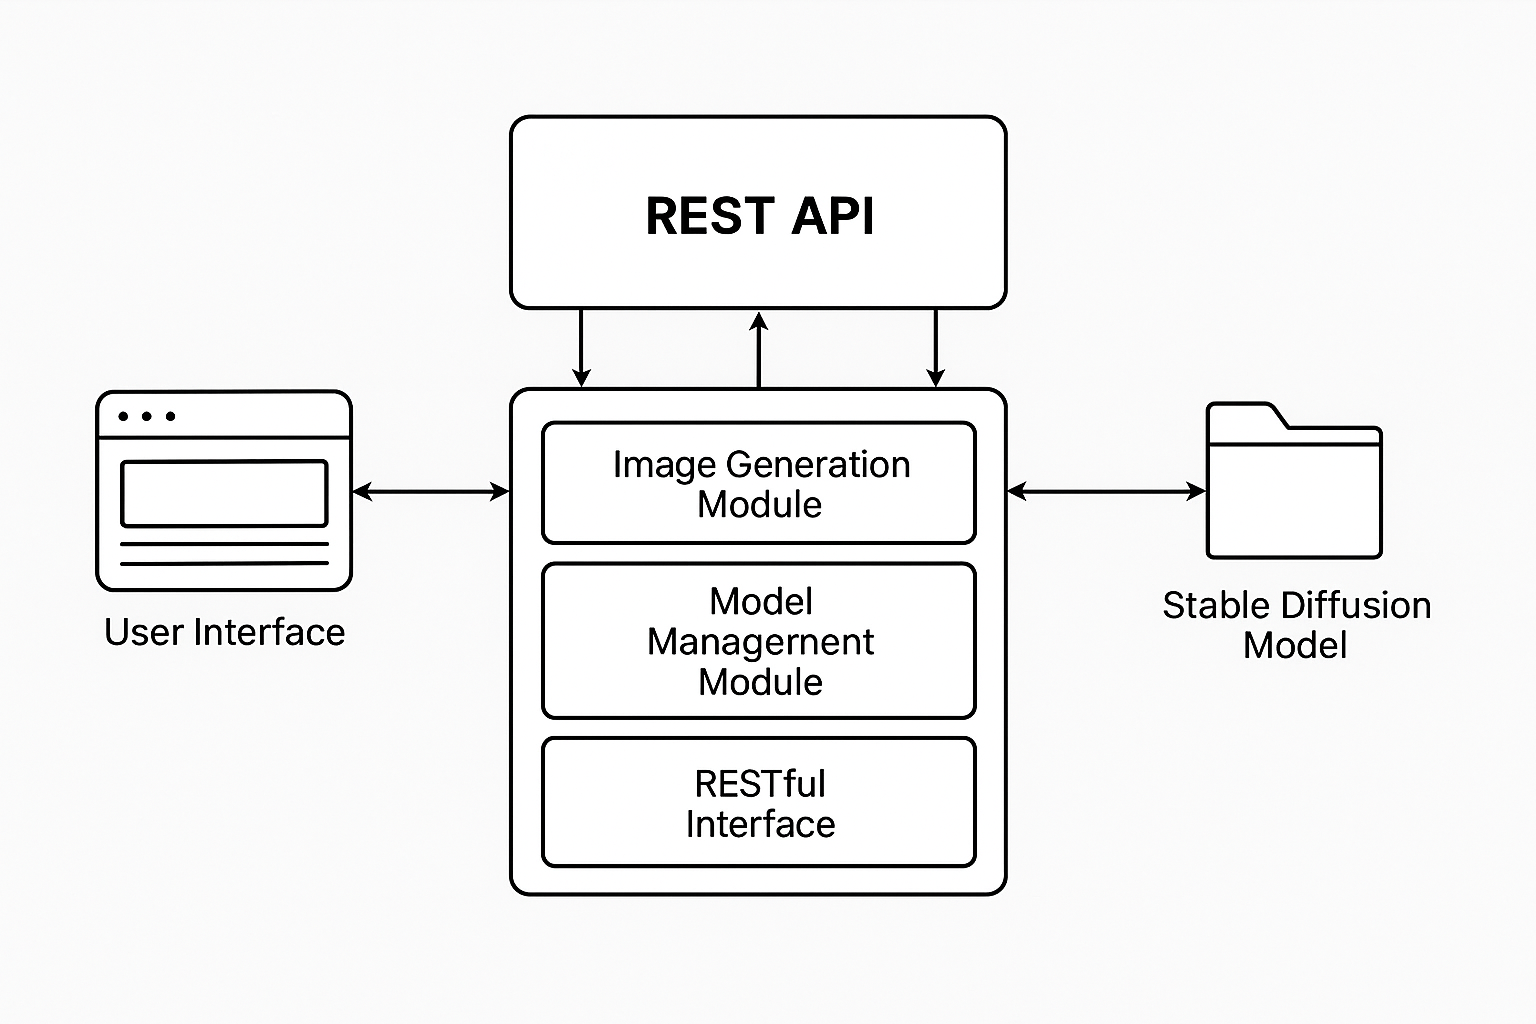
\includegraphics[width=0.6\textwidth]{diagramas/api_componentes.png}
\caption{Diagrama de componentes de la API generativa}
\label{fig:api-componentes}
\end{figure}

\subsubsection{Endpoints implementados} 
\paragraph{Generación de imágenes}
\begin{itemize}
    \item \textbf{POST /images/generate/}
    \begin{itemize}
        \item \textbf{Descripción:} genera una imagen a partir de una descripción textual.
        \item \textbf{Entrada (JSON):}
            \begin{itemize}
                \item \texttt{model\_name} (opcional, por defecto \texttt{stable\_modified})
                \item \texttt{prompt} (requerido)
                \item \texttt{num\_inference\_steps} (opcional, por defecto 50)
                \item \texttt{guidance\_scale} (opcional, por defecto 7.5)
            \end{itemize}
        \item \textbf{Salida:} JSON con la ruta de la imagen generada.
    \end{itemize}

    \item \textbf{GET /images/download/\{image\_name\}}
    \begin{itemize}
        \item \textbf{Descripción:} descarga una imagen generada.
        \item \textbf{Entrada:} nombre del archivo.
        \item \textbf{Salida:} archivo binario de imagen.
    \end{itemize}
\end{itemize}

\paragraph{Gestión de modelos}
\begin{itemize}
    \item \textbf{POST /models/upload/}
    \begin{itemize}
        \item \textbf{Descripción:} permite subir un nuevo modelo en formato ZIP.
        \item \textbf{Entrada:} archivo ZIP.
        \item \textbf{Salida:} JSON de confirmación y ruta del modelo.
    \end{itemize}

    \item \textbf{DELETE /models/delete/\{model\_name\}}
    \begin{itemize}
        \item \textbf{Descripción:} elimina un modelo previamente subido.
        \item \textbf{Entrada:} nombre del modelo.
        \item \textbf{Salida:} mensaje de confirmación.
    \end{itemize}

    \item \textbf{GET /models/list/}
    \begin{itemize}
        \item \textbf{Descripción:} devuelve un listado de todos los modelos disponibles.
        \item \textbf{Entrada:} ninguna.
        \item \textbf{Salida:} JSON con los nombres de los modelos.
    \end{itemize}
\end{itemize}

\begin{figure}[H]
\centering
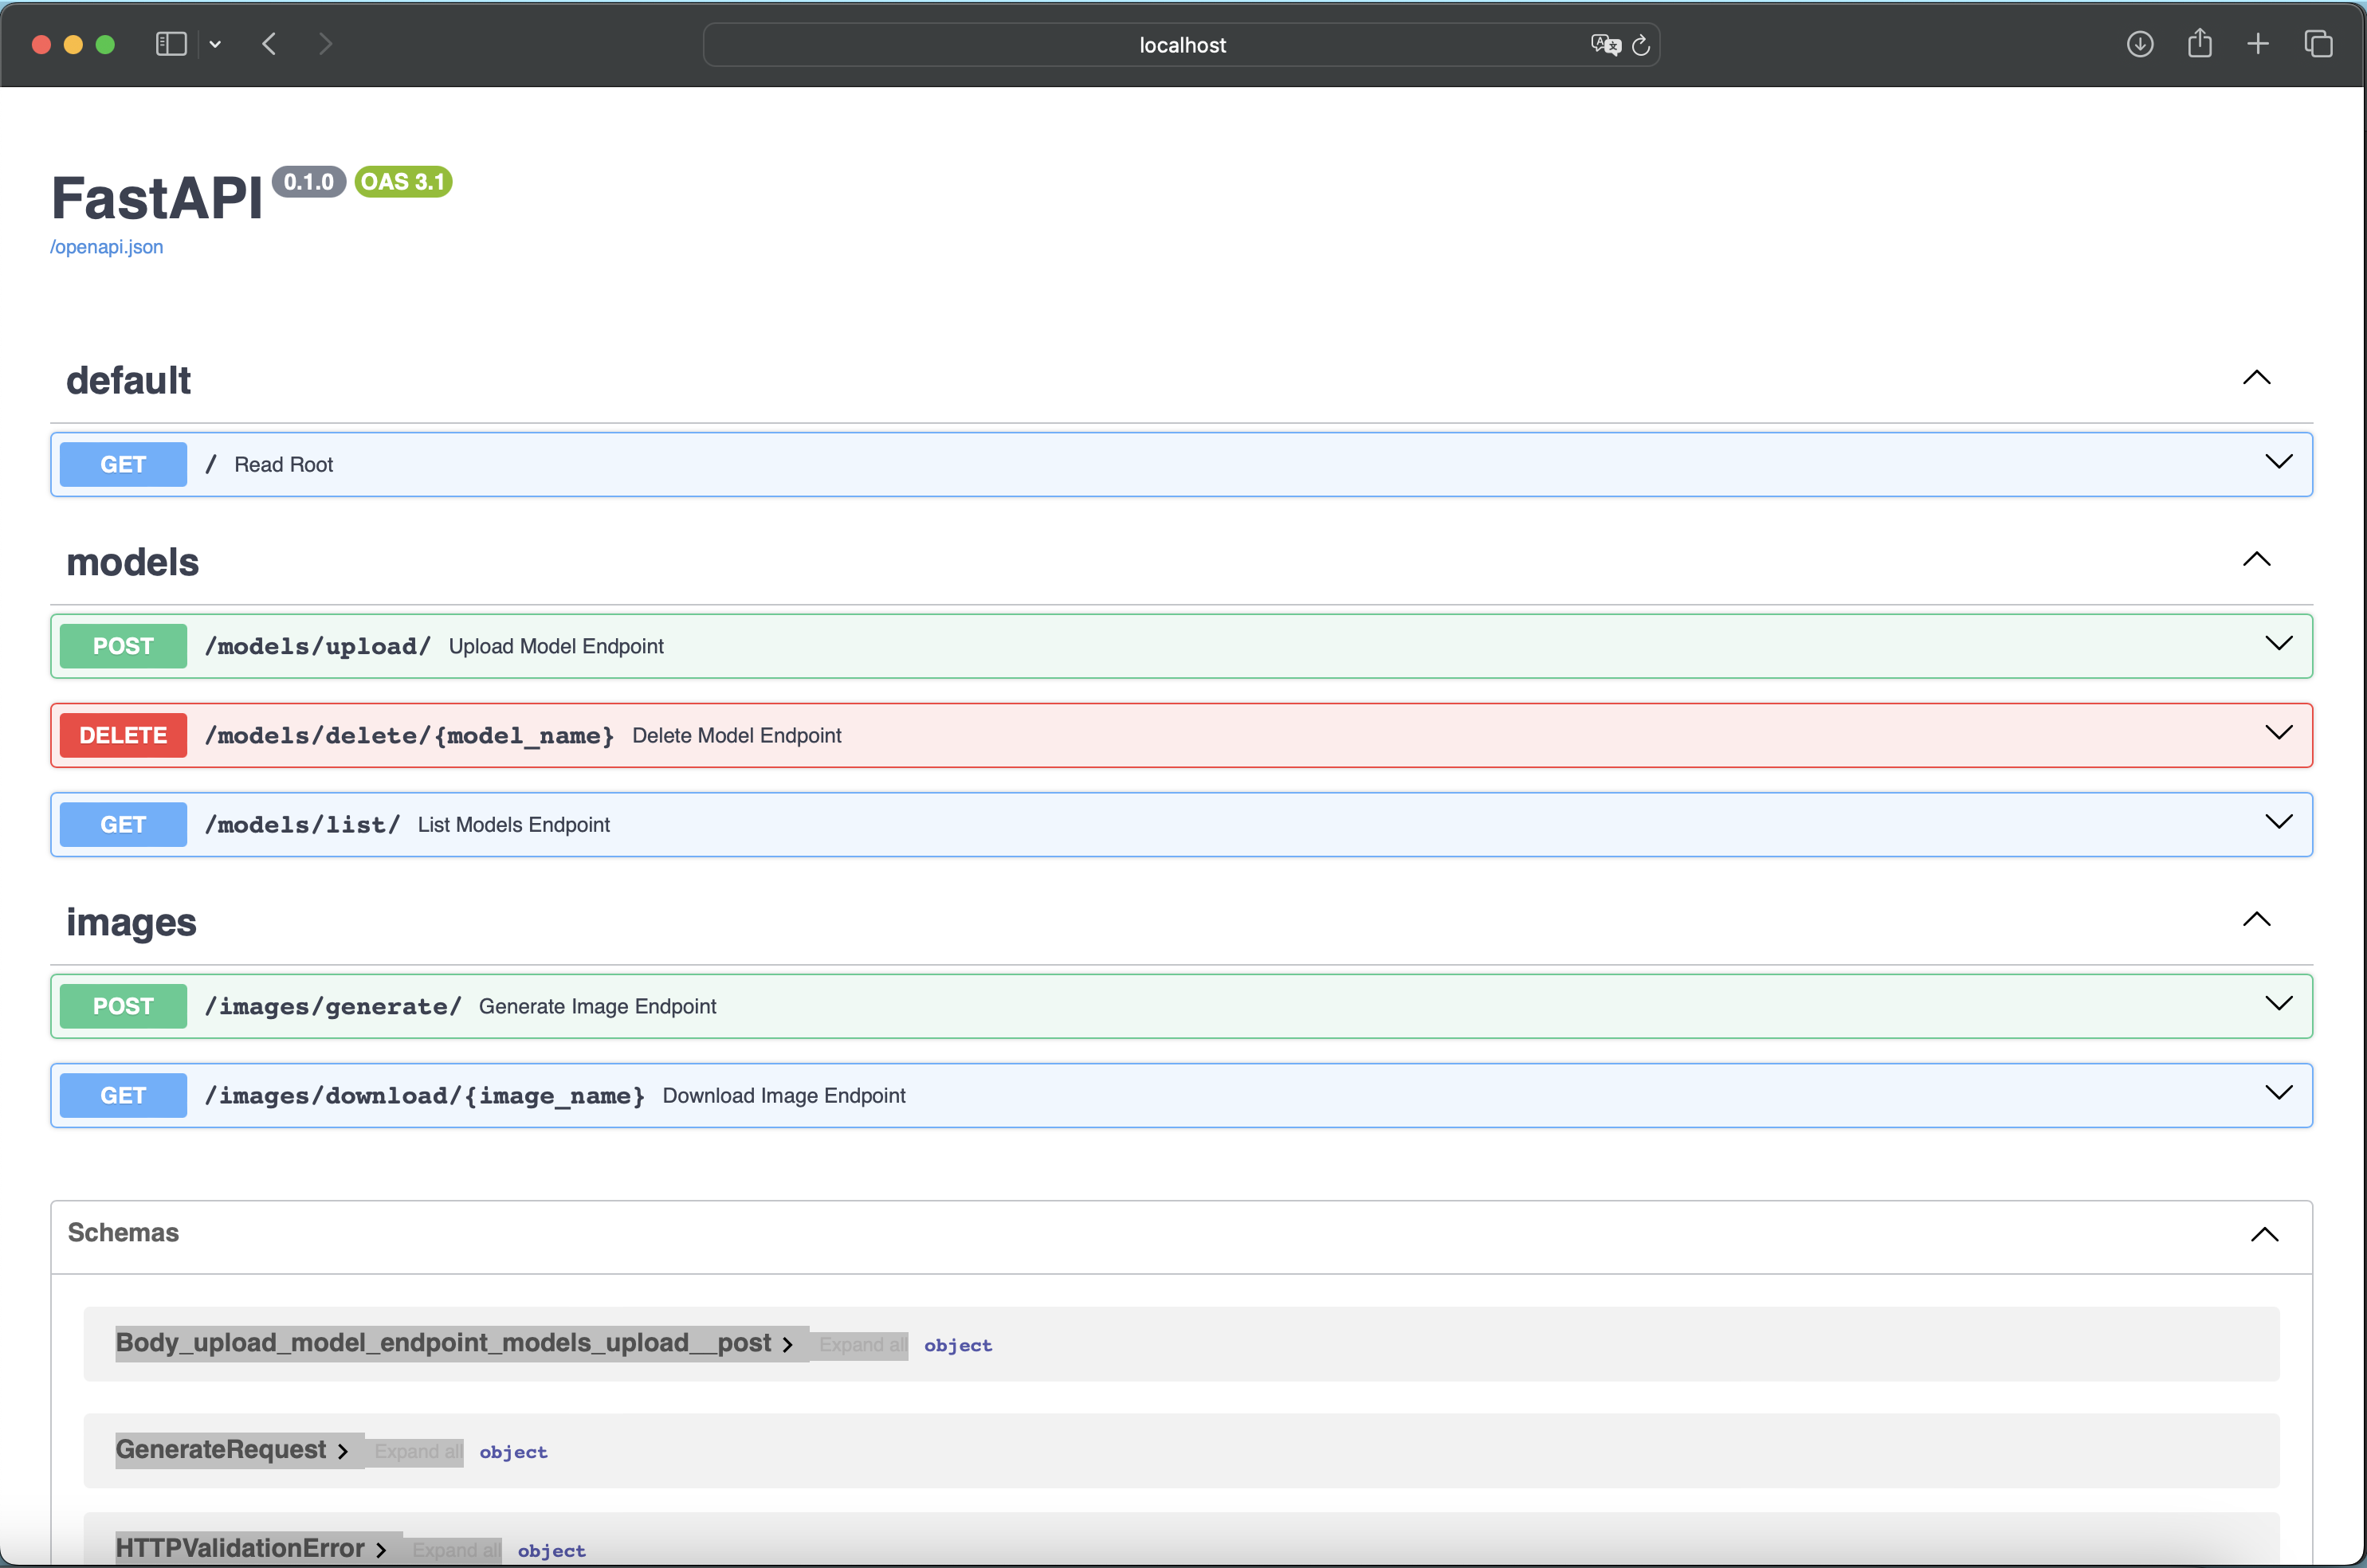
\includegraphics[width=0.5\textwidth]{api/vision_general.png}
\caption{Endpoints de la API generativa}
\label{fig:api-endpoints}
\end{figure}

\subsubsection{Flujo de interacción}

El flujo de uso parte de una descripción textual introducida en la interfaz de JMR. Esta se envía a través de un endpoint POST a la API, que responde con una imagen generada. La API también permite cambiar o cargar nuevos modelos desde la interfaz gráfica de la plataforma, lo que facilita la gestión dinámica sin necesidad de reiniciar el sistema.

\subsubsection{Entorno y despliegue}

La API se ejecuta en contenedores Docker configurados para su despliegue local. Esta elección permitió realizar pruebas aisladas, reproducibles y sin afectar al sistema anfitrión. Gracias a esta arquitectura, la API puede integrarse fácilmente en entornos más complejos como Kubernetes, o adaptarse para ejecutarse en servidores dedicados con balanceo de carga.

\subsubsection{Conclusión}
La API desarrollada con FastAPI proporciona una interfaz robusta y extensible para la generación de imágenes a partir de texto. Su diseño modular, combinado con validaciones estructurales y la posibilidad de gestionar modelos dinámicamente, garantiza una base sólida sobre la que seguir evolucionando el sistema. Aunque aún quedan aspectos por reforzar en seguridad y escalabilidad, la solución actual cumple eficazmente su propósito en entornos de desarrollo y validación funcional.